\documentclass[twocolumn]{article}
\usepackage{geometry}	%
\geometry{margin=2cm}	%more visible figures (more place) 
\usepackage[utf8]{inputenc}
\usepackage[english]{babel}
\usepackage{amsmath}	%booklet
\usepackage{hyperref}	%clickable citings, referencing URL via \url{}
\usepackage{siunitx}	%for SI units; see ftp://ftp.dante.de/tex-archive/macros/latex/exptl/siunitx/siunitx.pdf
\usepackage{graphicx} 	%includegraphics
\usepackage{mhchem}		%writing chemical elements with mass numbers
\usepackage[nottoc]{tocbibind}	%references
\usepackage{indentfirst}%indenting first paragraphs

%the command \insertFigure{file} inserts figure with width 0.9*(column width)
\newcommand{\insertFigure}[1]{%
   \includegraphics[width=0.9\linewidth]{#1}%
}

\title{K223}
\begin{document}
\maketitle
\newpage
\section{Introduction}
In order to conserve angular momentum, the probability that a nucleus relaxing toward the ground state will emit a photon in a given direction is dependent on the angle between the direction of emission and the spin axis of the nucleus \cite{sieg}. When studying a free nucleus, the nuclear spin axis is free to rotate in space and thus $\gamma$ emissions are isotropic. If relaxation proceeds through successive $\gamma$ emissions however, the two emissions will be angularly correlated if there isn't enough time for the projection of the nuclear spin to be perturbed and rotated by extra-nuclear fields in between the two emissions. The aim of this paper is to verify the angular correlation expected from the $\gamma$-$\gamma$ cascade of decaying $\ce{_27^{60}Co}$. To do so, a FAST-SLOW coincidence circuit was initially set up and the $\gamma$ spectrum of a $\ce{_27^{60}Co}$ sample was measured. The number of angularly correlated photons for different angles were then measured.
\section{Theory}
A detailed treatment of the theory of the angular correlation of nuclear radiation is provided in chapter XIX of \cite{sieg}. Figure \ref{fig:cobalt_scheme} shows the decay scheme of the sample used. The $\ce{_27^{60}Co}$ with half-life of $\approx 5.3$ years decays via $\beta^-$-radiation into $\ce{_28^{60}Ni}$ with highest probability to the $4^+$ angular momentum state. The $\ce{Ni}$ then relaxes to the ground state with the largest branching ratio being the $4^+\rightarrow2^+\rightarrow 0^+$ decay, producing two $\gamma$ photons with respective energies of 1.17 and 1.33~MeV. The lifetime of the intermediate $2^+$ $\ce{Ni}$ state is on the order of $\SI{1}{\pico\second}$ which is too short to be perturbed by extra-nuclear fields and thus allowing for the angular correlation treatment.
\begin{figure}[!h]
\centering
\insertFigure{cobalt_scheme.png}
\caption{$\ce{_27^{60}Co}$ decay scheme \cite{cobalt_scheme}}
\label{fig:cobalt_scheme}
\end{figure}
As the direction of the emission of the first photon is encoded with information on the projection of the spin axis of the nucleus due to angular momentum conservation, the probability of the direction of emission of the second photon depends on the direction of the first emission. Thus, there is an angular correlation between the directions of the two $\gamma$ emissions, given by the following directional correlation function for the $\gamma$-$\gamma$ cascade herein considered:
\[W(\theta) = 1+A_{22}P_2(\cos{\theta})+A_{44}P_4(\cos{\theta}),\] \label{eq:corr}
where $P_2$ and $P_4$ are Legendre Polynomials, $A_2 = 0.1020$, and $A_4 = 0.0091$ \cite{sieg}. This is the relation that will be tested in this paper.

\section{Experimental setup}
The design of the apparatus is shown in Figure \ref{fig:exp_setup}. 
\begin{figure}[!h]
	\centering
	\insertFigure{k223_setup.png}
	\caption{Experimental setup \cite{booklet}}
	\label{fig:exp_setup}
\end{figure}
\par The slow circuits count the number of photons incident to the respective detectors which have energies within energy range set by the respective single channel analyzers. This circuit is used to only count the number of incident $\gamma$~photons from the relevant $\gamma$-$\gamma$ cascade. The fast coincidence circuit counts the number of pairs of photons which arrive at the two detectors within a time window set by the fast coincidences unit. This circuit is used to distinguish and count pairs of photons which come from single $\gamma$-$\gamma$ cascade events as opposed to pairs of photons from two different cascade events. Though some random coincidences are still inevitably measured due to the large number of $\gamma$-$\gamma$ cascade events occurring at a given time in the sample, these random coincidences are eventually accounted for, as will be discussed in Section~\ref{sec:acc}. The number of coincident photons from the fast and slow circuits are then matched by the universal coincidence unit to count the number of pairs of photons with the right energies and within the right time frame to be labelled as coming from single $\gamma$-$\gamma$ cascade events.

\subsection{Detector}
The detectors consist of a crystal scintillator and a photomultiplier as show in Figure~\ref{fig:pmt}. The scintillator absorbs the $\gamma$-ray and re-emits visible light in form of scintillation, which induces electron emission in the photomultiplier (\textbf{PMT}) via the photoelectric effect. The high voltage provided between the photo-cathode and the anode accelerates the electron, which induces an avalanche of electrons by colliding with each of the dynodes. The signal produced by the \textbf{PMT} has a measurable height which is proportional to the energy of the incident photon. This signal is then input to the constant fraction discriminator in the fast circuit to measure the arrival time of the incident photon. As this procedure distorts the signal shape, which is required for the measurement of the energy of the incident photon, the output pulse cannot be used to measure the energy. Instead, an undistorted signal from an earlier phase of the amplification process is used as the input for the single channel analyzer (\textbf{SCA}) in the slow circuit.
\begin{figure}[!h]
	\centering
	\insertFigure{pmt.png}
	\caption{Scintillation detector with photomultiplier \cite{pmt}} 
	\label{fig:pmt}
\end{figure} 
\par One should note that Compton scattering also occurs in the scintillator when incident photons scatter inelastically inside the crystal instead of being absorbed. Scintillation photons are then produced with lower energy than those produced via absorption. This creates a Compton plateau spectrum bordered by two peaks on either side, as seen in Figure~\ref{fig:Compt}. The Compton edge is caused by the photons backscattering in the crystal, depositing the maximum of energy in the crystal from Compton scattering. The backscattered peak is instead caused by photons scattering back into the detector from the lead casing of the detector, with a large loss of energy, and then being absorbed by the crystal~\cite{Compton}. Though Compton scattering distorts the measure energy spectrum, the peaks from the absorbed photons should still be easily discernible at higher frequencies, visible in Figure~\ref{fig:Compt}.
\begin{figure}[!h]
\centering
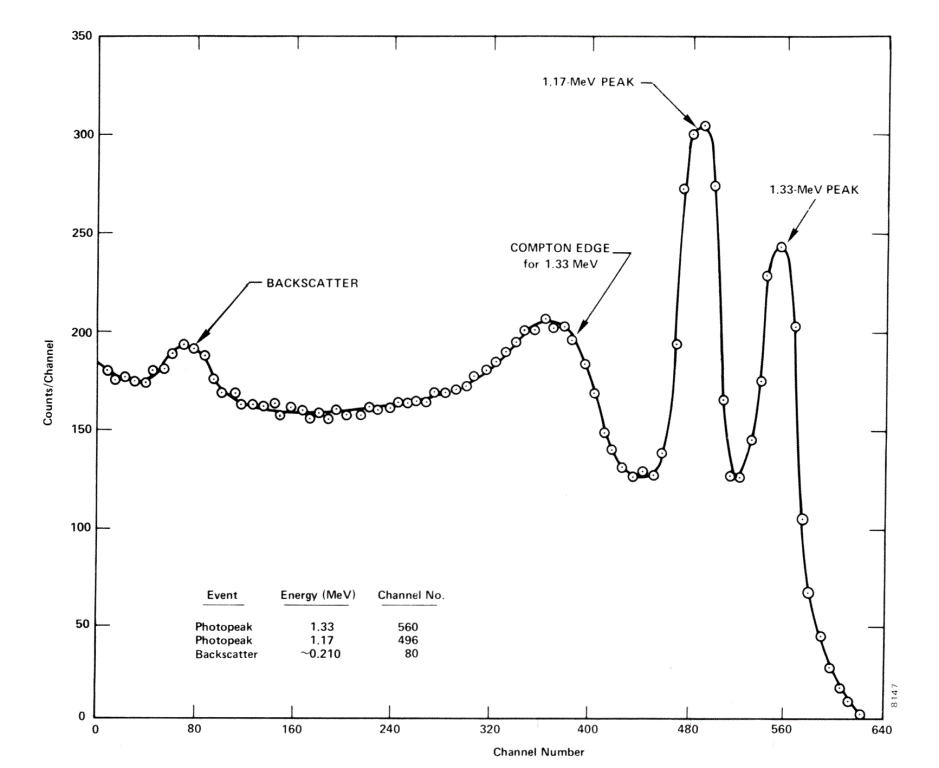
\includegraphics[width=1\linewidth]{Compt.png}
\caption{Compton scattering in the $\ce{^{60}Co}$ $\gamma$-$\gamma$ cascade spectrum \cite{Compt}} 
\label{fig:Compt}
\end{figure}

\subsection{Constant Fraction Discriminator}
%The fast coincidence circuit checks whether the two detected photons come from the same decay process. 
The constant fraction discriminators modify the signals as seen in Figure~\ref{fig:cfd}: an attenuated inverted copy of the input is added to the delayed input signal. The resulting shape crosses the $\SI{0}{\volt}$ line ("zero crossing point"). This point serves as a time stamp for the signal which does not depend on the amplitude of the signal.
\begin{figure}[!h]
	\centering
	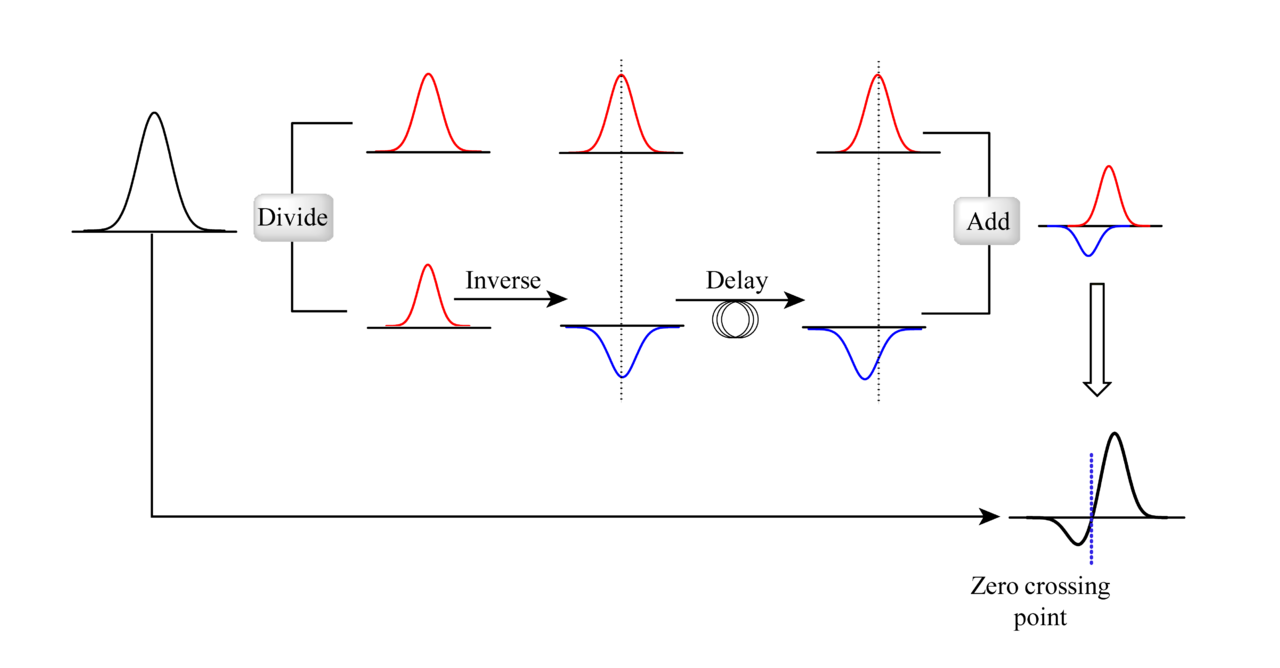
\includegraphics[width=1.02\linewidth]{cfd.png}
	\caption{Scintillation detector with photomultiplier \cite{cfd}} 
	\label{fig:cfd}
\end{figure}
The discriminator has two outputs: the "fast" output which is a negative digital pulse and the "slow" output which is a positive one. The latter is used by the fast coincidence unit \textbf{FC}.

%TODO is the original signal truly delayed, or is it the inverted signal? Could provide self-made figure. No this is right!
%TODO is it important to talk about the two different outputs of the CFD

\subsection{Single Channel Analyzers}
The weak, undistorted detector signal coming from the \textbf{PMT} is fed through the amplifiers \textbf{A1} and \textbf{A2} first. The analyzers \textbf{SCA1} and \textbf{SCA2} determine whether the amplitudes of the signals, which are proportional to the energy of the detected $\gamma$~photons, fall into an interval set by the \textbf{SCA}s. The interval is over a range of so-called channels of the \textbf{SCA} which are set either with upper and lower limit channels or with a lower limit and a window size.

\subsection{Universal coincidences}
The output signals from the \textbf{SCA}s and the \textbf{FC} are sent to the universal coincidence unit \textbf{UC} to count the total number of coincident photons within a time span set by the timer. The signals from the \textbf{SCA}s are first sent through delays to make sure the signals incident to the \textbf{UC} correspond to photons hitting both detectors at approximately the same time. The output from the \textbf{FC} is fed to a gate $\&$ delay generator \textbf{D$^2$-G$^2$} which delays the fast signal to ensure that the fast coincidences are correctly assigned to the same photons measured in the slow circuit when fed into the \textbf{UC}. Thus, the \textbf{UC} counts the total number of pairs of photons which have the right energy, and arrive within a short enough time frame, which is expected from $\gamma$-$\gamma$ cascade events.


\section{Procedure} \label{sec:Proc}
\subsection{Solid Angle Corrections}
\cite{sieg} provides solid angle correction factors $Q_2$ and $Q_4$ for detectors placed 5, 7, and 10~cm from the $\ce{^{60}Co}$ sample. These factors correct for the assumption made by the angular correlation function equation~\ref{eq:corr} that the detectors are point-like though indeed they are not. The closer the detectors are placed to the source, the larger the solid angle of the detectors become and thus the uncertainty introduced from the fact that they do not simply measure counts for a single angle is increased. That said, the further away the detectors are placed from the source, the smaller the photon count rate becomes for a given time span which increases the relative uncertainty of the count rate (as photon emissions follow Poisson statistics). Rough measurements were taken for different detector placements to estimate the expected uncertainty introduced by photon counts for the angular correlation measurements. It was decided to place the detectors 7~cm away from the source in order to minimise uncertainty, though whether this is indeed the best placement cannot be known due to the unknown nature of the uncertainty introduced by the solid angle correction. As the solid angle correction factors depend on the energy of the incident photons and \cite{sieg} only provides correction factors for energies of 0.5, 1.0, and 1.5~MeV, linear interpolation was utilised to obtain factor values for our photons which have energies of 1.17 and 1.33~MeV and thus a mean of $E_{\text{avg}} = 1.252$~MeV. The factor values obtained are,
\begin{align*}
&Q_2\big(E_{\text{avg}}\big) \equiv Q^*_2 = 0.9623,\\
&Q_4\big(E_{\text{avg}}\big) \equiv Q^*_4 = 0.8782.
\end{align*}
This method reduces the uncertainty caused by the energy dependence of the solid angle correction factors. That said, there is still a small uncertainty which remains caused by the different energies of the two cascade photons which would require individual correction factors, though we do not distinguish between the two different cascade photons during measurements in this experiment.
%TODO Make sure that the Q values aren't repeated in the results.

\subsection{Amplifiers, CFDs}
The amplifiers \textbf{A$_1$}, \textbf{A$_2$} were then adjusted. We changed the gain using an oscilloscope such that the peaks corresponding to different detected photon energy levels don't hit the $\SI{9}{\volt}$ output ceiling of the amplifiers. We set the maximum to approximately $\SI{8}{\volt}$. The result of the adjustment is shown in Figure \ref{fig:amp}. Next we set the threshold of constant-fraction discriminators above the noise level by using the output of the \textbf{CFD} as the trigger for the amplifier signal of the same detector, increasing the threshold until the bright line at $\SI{0}{\volt}$ showing no photon detection (e.g. noise) disappeared. 
%TODO which image, if any, shows the CFD output? Looking for channel 2-trigger.
\begin{figure}[!h]
	\centering
	\insertFigure{./screenshots/SC08_cropped.png}
	\caption{Well-adjusted signal of the first amplifier. A too high gain would cause the highest peaks to flatten due to saturation before the maximum.} 
	\label{fig:amp}
\end{figure}

\subsection{Prompt Curve}
We connected the positive outputs of the \textbf{CFD}s to the fast coincidence unit \textbf{FC}, one of them through a delay unit \textbf{D3}. While keeping the resolution time of the \textbf{FC} at $\SI{15}{\nano\second}$, which was a value approximately expected, we changed the delay of \textbf{D3} to measure the coincidental detections as a function of the delay. We measured the counts for $\SI[separate-uncertainty = true]{10.0(1) }{\second}$ for each delay value which was sufficient to plot an informative prompt curve, given in Figure~\ref{fig:prompt}.
\begin{figure}[!h]
	\centering
	\insertFigure{prompt_with_gauss.png}
	\caption{The measured prompt curve and a fitted Gaussian to quantify the width. The parameters are $\mu = \SI[separate-uncertainty = true]{11.1 \pm 0.9}{\nano\second}$ (mean), $\sigma = \SI[separate-uncertainty = true]{9.3 \pm 1.3}{\nano\second}$ (deviation), $A = 8259.8 \pm	881.8$ (scaling factor). Two measured values at 61 ($17 \pm 4.1$ counts) and 63~ns ($29 \pm 5.4$) are not shown.}
	\label{fig:prompt}
\end{figure}
From the figure, the count rate approximately plateaus from a delay of approximately 4~ns to 18~ns. This gives confidence in the resolution time of the \textbf{FC} set at $\SI{15}{\nano\second}$ when the delay of \textbf{D3} is set to 11~ns. These values were used for the angular correlation measurements. The Gaussian fitted post factum confirmed our choice ($\mu$), and provided the experimental resolving time of the fast coincidence circuit  $\text{FWHM} = 2 \sqrt{2 \text{ln}2} \sigma = \SI[separate-uncertainty = true]{21.9 \pm 3.0}{\nano \second}$\cite{signal}. A possible explanation to the discrepancy between the experimental and the set value ($15$ ns) might be the false assumption that the timing uncertainties of the two \textbf{CFD} units follow a normal distribution: in this case, the prompt curve would also be a Gaussian, instead of having a clearly visible plateau. 

\subsection{Energy Spectra}
The energy spectra from both detectors was plotted by scanning the entire relevant channels of both \textbf{SCA}s. The detectors were placed at 180$^{\circ}$ separation where the largest number of coincidence counts are theoretically expected. We again measured the counts for $\SI[separate-uncertainty = true]{10.0(1) }{\second}$, which was sufficient to obtain adequate spectra. A window size of 150 channels for both \textbf{SCA}s was used. Measurement were taken until the full spectrum expected from Figure~\ref{fig:Compt} was obtained for both detectors. The spectra are given in Figure~\ref{fig:spectra}.
\begin{figure}[!h]
	\centering
	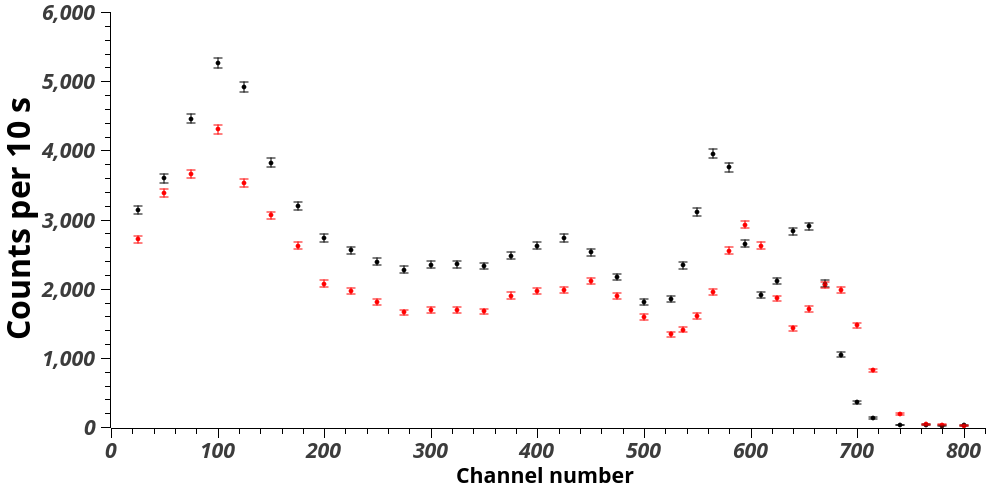
\includegraphics[width=0.9\linewidth]{detectors2.png}
	\caption{Measured energy spectra of both detectors.}
	\label{fig:spectra}
\end{figure}
The two $\gamma$-$\gamma$ cascade photon peaks are clearly visible for both detectors at the upper end of the spectra, as well as the backscatter peaks at the lower end of the spectra and Compton edges around channel 450. The channel windows chosen for \textbf{SCA1} and \textbf{SCA2} were 520--720 and 540--740 respectively, in order to include both $\gamma$-$\gamma$ cascade photon peaks.

\subsection{Accidental Coincidences} \label{sec:acc}
Two photons might be detected as coincidental yet come from two different atoms, we need to take this noise into account. We measured the accidental coincidences overnight, and during the length of $\SI{59820}{\second}$, $21855 \pm 148$ coincidences were recorded, which corresponds to $146.14 \pm 0.99$ counts over $\SI{400}{\second}$, or $0.3653 \pm 0.0025$
counts each second. The individual \textbf{SCA} units measured $260560000 \pm 16142$ and $243720000 \pm 15612$ incoming photons within the correct energy interval, or
 \begin{equation}
 N_{\text{SCA 1}} = 4355.73 \pm 0.27 \hspace{8pt} \text{and} \hspace{8pt} N_{\text{SCA 2}} =  4074.22 \pm 0.26 \nonumber
 \end{equation}
 each second. Using the time resoultion $\sigma = \SI[separate-uncertainty = true]{21.9 \pm 3.0}{\nano \second}$ of the \textbf{FCC} (see Figure \ref{fig:prompt}), we can calculate the expected accidental coincidences (see \cite{leo} for a detailed explanation) as
\begin{equation}
N_{\text{acc}} = \sigma \cdot N_{\text{SCA 1}} \cdot N_{\text{SCA 2}} = 0.3886 \pm 0.0532 \nonumber
\end{equation}
counts per second, which agrees with the experimental results.
\begin{figure}
\centering
\insertFigure{./screenshots/SC07_cropped.png}
\caption{Adjusting the delay of the SCAs such that the leading edges of the signals from one SCA (yellow) and the gate and delay generator coincide.}
\label{fig:sca-overlap}
\end{figure}

\section{Results}
\subsection{Angular correlation}
We tried fitting a function of the form~\cite{sieg}
\begin{equation}
W(\theta) = A \big(1 + B (Q^{*}_2)^2 \cos^2 \theta + C (Q^{*}_4)^2 \cos^4 \theta \big) \nonumber
\end{equation} 
using the least-squares-fit method, which produced
\begin{align*}
&A = 3602.14 \pm 40.01\\
&B = 0.1157  \pm 0.0660\\
&C = 0.04035 \pm 0.07465
\end{align*}
%TODO only give two sig figs for the uncertainty then give values to that decimal point.
The theoretical values of $B$ and $C$ ($A$ is a scaling factor depending on the measurement time):
\begin{align*}
&B_{\text{th}} = \frac{1}{8} = 0.125\\
&C_{\text{th}} = \frac{1}{24} = 0.041\bar{6}
\end{align*}
\section{Conclusion}
We set up an experiment to analyze the angular correlation of the $\gamma$-$\gamma$ cascade in a $\ce{_27^{60}Co}$ sample. We achieved a somewhat good agreement with the theoretical prediction, and the main source of the errors can be easily identified: a longer measurement time would have allowed for smaller relative uncertainties, as visible in the case of the overnight recording of the accidental coincidences.

\begin{figure}
	\centering
	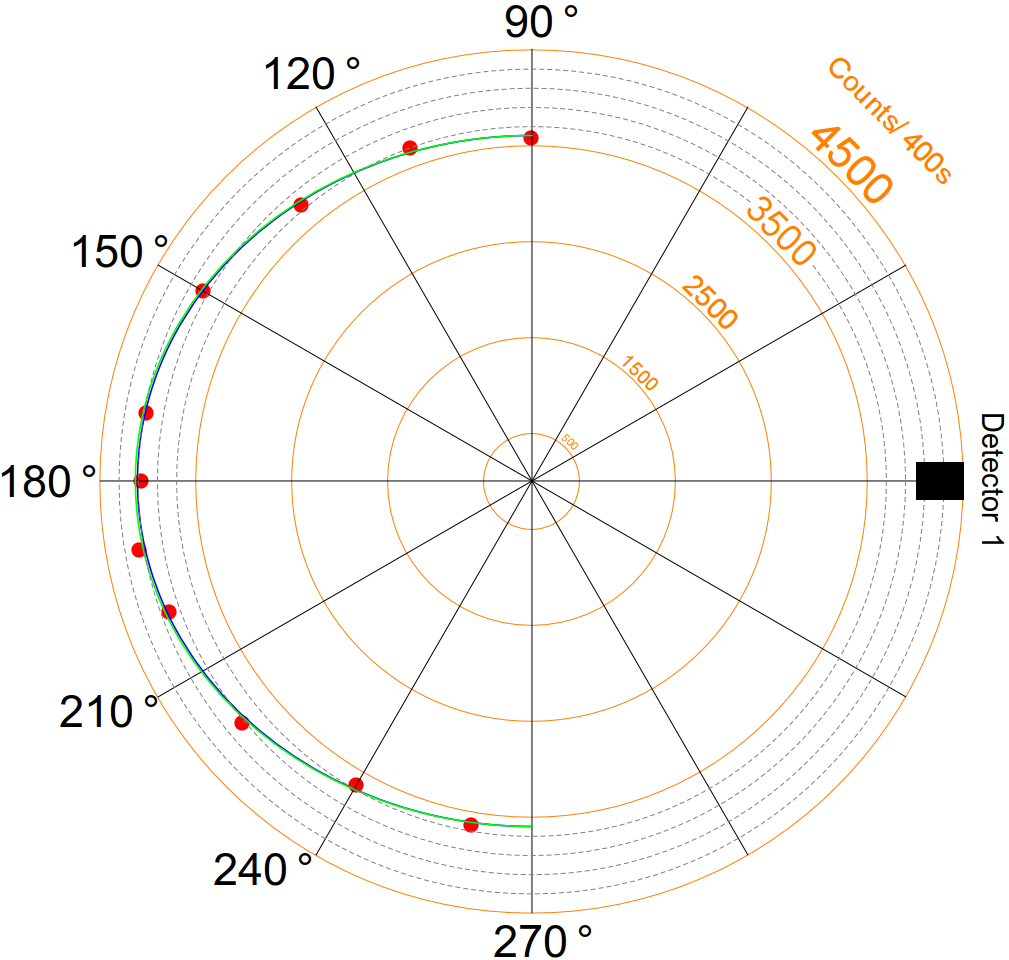
\includegraphics[width=\linewidth]{polar2.png}
	\caption{Polar plot of the counts against angle. Uncertainties are not displayed for the measurements. The weighted fit is given in blue, the theoretical result in green.}
	\label{fig:polar}
\end{figure}

\begin{thebibliography}{9}

%TODO order bibliography by order of appearance
\bibitem{sieg}
Siegbahn, K.: Alpha-, beta-, and gamma-ray spectroscopy, Vol. 2, North Holand Publishing Company, Amsterdam, 1965.
\bibitem{booklet}
Unspecified author: Advanced Laboratory Course (physics601) Description of Experiments, University of Bonn, 2018.
\bibitem{cobalt_scheme}
R. B. Firestone, Table of Isotopes $8$\textsuperscript{th} edition
 (Wiley, New York, 1996)
 \bibitem{pmt}
 \url{http://wanda.fiu.edu/teaching/courses/Modern_lab_manual/scintillator.html}
\bibitem{cfd}
\url{https://en.wikipedia.org/wiki/Constant_fraction_discriminator#/media/File:Operation_of_a_CFD.png}
%alternative url: https://en.wikipedia.org/wiki/Constant_fraction_discriminator
\bibitem{signal}
Nakhostin: Signal Processing for Radiation Detectors, Wiley (2018)
%Mohammad Nakhostin
\bibitem{Compt}
\url{https://www.nuclear-power.net/nuclear-power/reactor-physics/interaction-radiation-matter/interaction-gamma-radiation-matter/compton-scattering/compton-edge}
\bibitem{Compton}
\url{https://www.phys.ufl.edu/courses/phy4803L/group_I/gamma_spec/gamspec.pdf}
\bibitem{leo}
William R. Leo: Techniques for Nuclear and Particle Physics Experiments, Springer-Verlag (1987)
%TODO check for correctness of these book details
\end{thebibliography}
\end{document}